\documentclass[border=2pt]{standalone}
\usepackage{graphicx,newtxtext}
\begin{document}
\begin{minipage}{420pt}\centering
\begin{minipage}[t]{.322\linewidth}\centering
\vspace{0pt}\begin{minipage}[c][88pt][c]{\linewidth}\centering
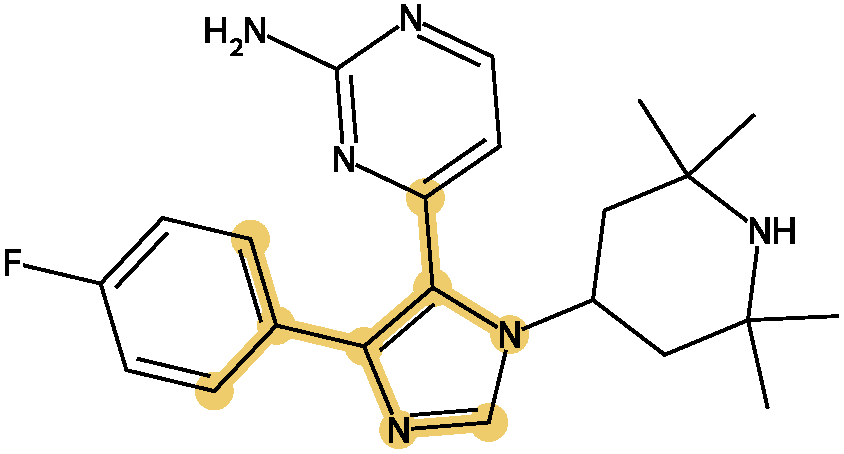
\includegraphics[width=\linewidth,height=88pt,keepaspectratio]{bit204.pdf}
\end{minipage}\par\smallskip
{\fontsize{9}{10}\selectfont (a) Substituted imidazole\\junction (bit 204)\par}
{\fontsize{8}{10}\selectfont SB-221466 (CHEMBL95502)\par}
\end{minipage}\hfill
\begin{minipage}[t]{.322\linewidth}\centering
\vspace{0pt}\begin{minipage}[c][88pt][c]{\linewidth}\centering
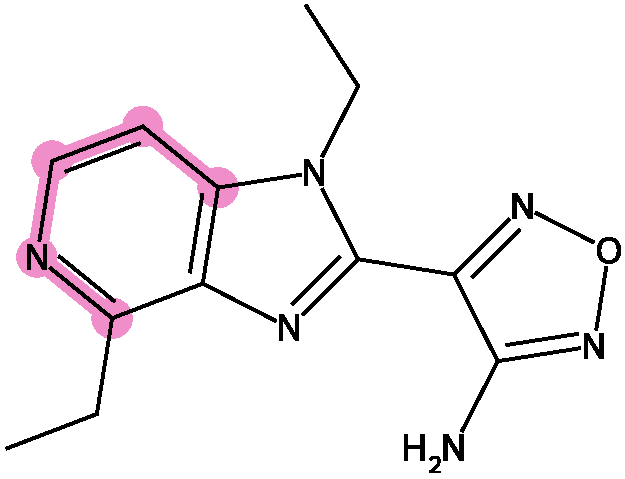
\includegraphics[width=\linewidth,height=88pt,keepaspectratio]{bit19.pdf}
\end{minipage}\par\smallskip
{\fontsize{9}{10}\selectfont (b) Pyridine-ring segment\\(bit 19)\par}
{\fontsize{8}{10}\selectfont SB-751148 (CHEMBL365072)\par}
\end{minipage}\hfill
\begin{minipage}[t]{.322\linewidth}\centering
\vspace{0pt}\begin{minipage}[c][88pt][c]{\linewidth}\centering
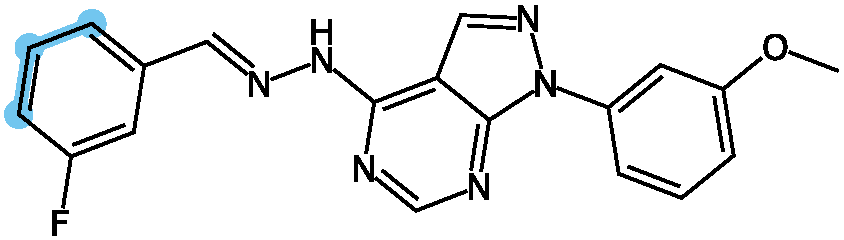
\includegraphics[width=\linewidth,height=88pt,keepaspectratio]{bit64.pdf}
\end{minipage}\par\smallskip
{\fontsize{9}{10}\selectfont (c) Aromatic carbon\\environment (bit 64)\par}
{\fontsize{8}{10}\selectfont CHEMBL69757\par}
\end{minipage}
\end{minipage}\end{document}
